\documentclass[12pt, leqno]{article} %% use to set typesize
\include{common}

\begin{document}

\hdr{2019-10-07}

\section{Householder transformations}

The Gram-Schmidt orthogonalization procedure is not generally
recommended for numerical use.  Suppose we write $A = [a_1 \ldots
  a_m]$ and $Q = [q_1 \ldots q_m]$.  The essential problem is that if
$r_{jj} \ll \|a_j\|_2$, then cancellation can destroy the accuracy of
the computed $q_j$; and in particular, the computed $q_j$ may not be
particularly orthogonal to the previous $q_j$.  Actually, loss of
orthogonality can build up even if the diagonal elements of $R$ are
not exceptionally small.  This is Not Good, and while we have some
tricks to mitigate the problem, we need a different approach if we
want the problem to go away.

Recall that one way of expressing the Gaussian elimination algorithm
is in terms of Gauss transformations that serve to introduce zeros
into the lower triangle of a matrix.  {\em Householder} transformations
are orthogonal transformations (reflections) that can be used to similar
effect.  Reflection across the plane orthogonal to a unit normal
vector $v$ can be expressed in matrix form as
\[
  H = I-2 vv^T.
\]

Now suppose we are given a vector $x$ and we want to find a reflection
that transforms $x$ into a direction parallel to some unit vector $y$.
The right reflection is through a hyperplane that bisects the angle
between $x$ and $y$ (see Figure~\ref{fig1}), which we can construct
by taking the hyperplane normal to $x-\|x\|y$.  That is,
letting $u = x - \|x\|y$ and $v = u/\|u\|$, we have
\begin{align*}
  (I-2vv^T)x
  & = x - 2\frac{(x+\|x\|y)(x^T x + \|x\| x^T y)}{\|x\|^2 + 2 x^T y \|x\| + \|x\|^2 \|y\|^2} \\
  & = x - (x-\|x\|y) \\
  & = \|x\|y.
\end{align*}
If we use $y = \pm e_1$, we can get a reflection that zeros out all but the
first element of the vector $x$.  So with appropriate choices of reflections,
we can take a matrix $A$ and zero out all of the subdiagonal elements
of the first column.

\begin{figure}
\begin{center}
  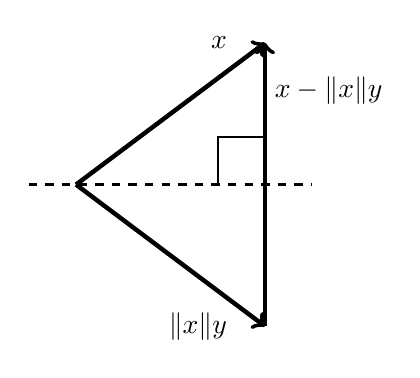
\begin{tikzpicture}[scale=0.6]
    \draw [thick,dashed] (-1,0) -- (5,0);
    \draw [ultra thick,->] (0,0) -- (4,3);
    \draw [ultra thick,->] (0,0) -- (4,-3);
    \draw [ultra thick,->] (4,-3) -- (4,3);
    \draw [thick] (3,0) -- (3,1) -- (4,1);
    \draw (4,2) node [right] {$x-\|x\| y$};
    \draw (3.4,3) node [left] {$x$};
    \draw (3.4,-3) node [left] {$\|x\| y$};
  \end{tikzpicture}
\end{center}
\caption{Construction of a reflector to transform $x$ into $\|x\|y$,
         $\|y\| = 1$.}
\label{fig1}
\end{figure}

Now think about applying a sequence of Householder transformations to
introduce subdiagonal zeros into $A$, just as we used a sequence of Gauss
transformations to introduce subdiagonal zeros in Gaussian elimination.
This leads us to the following algorithm to compute the $QR$
decomposition:
\lstinputlisting{code/hqr1.m}
Note that there are two valid choices of $u_1$ at each step;
we make the choice that avoids cancellation in the obvious version
of the formula.

As with $LU$ factorization, we can re-use the storage of $A$ by recognizing
that the number of nontrivial parameters in the vector $w$ at each step
is the same as the number of zeros produced by that transformation.
This gives us the following:
\lstinputlisting{code/hqr2.m}

If we ever need $Q$ or $Q^T$ explicitly, we can always form it from
the compressed representation.  We can also multiply by $Q$ and $Q^T$
implicitly:
\lstinputlisting{code/applyQ.m}
\lstinputlisting{code/applyQT.m}

\section{Givens rotations}

Householder reflections are one of the standard orthogonal
transformations used in numerical linear algebra.  The other standard
orthogonal transformation is a {\em Givens rotation}:
\[
  G = \begin{bmatrix}
    c & -s \\
    s & c
  \end{bmatrix}.
\]
where $c^2 + s^2 = 1$.  Note that
\[
  G = \begin{bmatrix}
    c & -s \\
    s & c
  \end{bmatrix}
  \begin{bmatrix}
    x \\ y
  \end{bmatrix} =
  \begin{bmatrix}
    cx - sy \\
    sx + cy
  \end{bmatrix}
\]
so if we choose
\begin{align*}
  s &= \frac{-y}{\sqrt{x^2 + y^2}}, &
  c &= \frac{x}{\sqrt{x^2+y^2}}
\end{align*}
then the Givens rotation introduces a zero in the second column.
More generally, we can transform a vector in $\bbR^m$ into a vector
parallel to $e_1$ by a sequence of $m-1$ Givens rotations, where
the first rotation moves the last element to zero, the second rotation
moves the second-to-last element to zero, and so forth.

For some applications, introducing zeros one by one is very
attractive.  In some places, you may see this phrased as a contrast
between algorithms based on Householder reflections and those based on
Givens rotations, but this is not quite right.  Small Householder
reflections can be used to introduce one zero at a time, too.
Still, in the general usage, Givens rotations seem to be the more
popular choice for this sort of local introduction of zeros.

\section{Stability of QR}

It is not too difficult to show that applying a Givens rotations or
Householder reflector to a matrix is backward-stable: if $P$ is the
desired transformation, the floating point result of $PA$ is
\[
  \tilde{P} A = (P+E) A, \quad \|E\| \leq O(\macheps) \|A\|.
\]
Moreover, orthogonal matrices are perfectly conditioned!
Taking a product of $j$ matrices is also fine; the result
has backward error bounded by $j O(\macheps) \|A\|$.
As a consequence, QR decomposition by Givens rotations or Householder
transformations is ultimately backward stable.

The stability of orthogonal matrices in general makes them a
marvelous building block for numerical linear algebra algorithms,
and we will take advantage of this again when we discuss
eigenvalue solvers.

\section{Sparse QR}

Just as was the case with LU, the QR decomposition admits a sparse
variant.  And, as with LU, sparsity of the
matrix $A \in \bbR^{m \times n}$ alone is not
enough to guarantee sparsity of the factorization!  Hence, as with
solving linear systems, our recommendation for solving sparse least
squares problems varies depending on the actual sparse structure.

Recall that the $R$ matrix in QR factorization is also the Cholesky
factor of the Gram matrix: $G = A^T A = R^T R$.  Hence, the sparsity of
the $R$ factor can be inferred from the sparsity of $G$ using the ideas
we talked about when discussing sparse Cholesky.  If the rows of $A$
correspond to experiments and columns correspond to factors, the nonzero
structure of $G$ is determined by which experiments share common
factors: in general $g_{ij} \neq 0$ if any experiment involves both
factors $i$ and factor $j$. So a very sparse $A$ matrix may nonetheless
yield a completely dense $G$ matrix. Of course, if $R$ is dense, that is
not the end of the world!  Factoring a dense $n \times n$ matrix is
pretty cheap for $n$ in the hundreds or even up to a couple thousand,
and solves with the resulting triangular factors are quite inexpensive.

If one forms $Q$ at all, it is often better to work with $Q$ as a
product of (sparse) Householder reflectors rather than forming the
elements of $Q$.  One may also choose to use a ``$Q$-less QR decomposition''
in which the matrix $Q$ is not kept in any explicit form; to form $Q^T b$
in this case, we would use the formulation $Q^T b = R^{-T} A^T b$.

As with linear solves, least squares solves can be ``cleaned up''
using iterative refinement.  This is a good idea in particular when
using $Q$-less QR.  If $\tilde{A}^\dagger$ is an approximate least
squares solve (e.g.~via the slightly-unstable normal equations approach),
iterative refinement looks like
\begin{align*}
  r^{k} &= b-Ax^{k} \\
  x^{k+1} &= x^k - \tilde{R}^{-1} (\tilde{R}^{-T} (A^T r_k)).
\end{align*}
This approach can be useful even when $A$ is moderately large and dense;
for example, $\tilde{R}$ might be computed from a (scaled) QR
decomposition of a carefully selected subset of the rows of $A$.

\section{Constrained case}

Consider the weighted least squares problem
\[
  \mbox{minimize } \sum_{i=1}^m w_i r_i^2
\]
where $w_1$ is much larger than the others.  If we
let $w_1 \rightarrow \infty$ while the others are fixed, what happens?
We essentially say that we care about enforcing the first equation
above all others, and in the limit we are solving the {\em constrained}
least squares problem
\[
  \mbox{minimize } \sum_{i=2}^m w_i r_i^2 \mbox{ s.t. } r_1 = 0.
\]
Unfortunately, if we actually try to compute this way, we are dancing on
dangerous ground; as $w_1$ goes to infinity, so does the condition
number of the least squares problem.  But this is only an issue with the
weighted formulation; we can formulate the constrained problem in other
ways that are perfectly well-behaved.

In the remainder of this section, we address two ways of handling
the linearly constrained least squares problem
\[
  \mbox{minimize } \|Ax-b\|^2 \mbox{ s.t. } C^T x = d,
\]
by either eliminating variables (the {\em null-space method}) or adding
variables (the method of {\em Lagrange multipliers}).

\subsection{Null space method}

In the null space method, we write an explicit expression for the solutions
to $C^T x = d$ in the form $x^p + W z$ where $x^p$ is a particular solution
to $C^T x^p = d$ and $W$ is a basis for the null space of $C^T$.  Perhaps the
simplest particular solution is $x^p = (C^T)^\dagger d$, the solution with
minimal norm; we can compute both
this particular solution and an orthogonormal null space basis quickly
using a full QR decomposition of $C$:
\[
  C =
    \begin{bmatrix} Q_1 & Q_2 \end{bmatrix}
    \begin{bmatrix} R_1 \\ 0 \end{bmatrix}, \quad
  x^p = Q_1 R_1^{-T} d, \quad W = Q_2.
\]
Note that
\[
  C^T x^p = (R_1^T Q_1^T) x^p = d,
\]
so this is indeed a particular solution.
Having written an explicit parameterization for all solutions of the
constraint equations, we can minimize the least squares objective with
respect to the reduced set of variables
\[
  \mbox{minimize } \|A(x^p + Wz) - b\|^2 = \|(AW)z - (b-Ax^p)\|^2.
\]
This new least squares problem involves a smaller set of variables
(which is good); but in general, even if $A$ is sparse, $AW$ will not be.
So it is appropriate to have a few more methods in our arsenal.

\subsection{Lagrange multipliers}

An alternate method is the method of {\em Lagrange multipliers}.
This is an algebraic technique for adding equations to enforce constraints.

One way to approach the Lagrange multiplier method is to look at the
equations for a constrained minimum.  In order not to have a downhill
direction, we require that the directional derivatives be zero in any
direction consistent with the constraint; that is, we require $Cx = d$
and
\[
  \delta x^T A^T r = 0 \mbox{ when } C^T \delta x = 0.
\]
The constraint says that admissible $\delta x$ are
orthogonal to the columns of $C$; the objective tells us the admissible
$\delta x$ should be orthogonal to the residual.  So we need that $A^T r$
should lie in the column span of $C$; that is,
\[
  A^T r = -C \lambda
\]
for some $\lambda$, and $Cx = d$.  Putting this together,
we have the KKT equations
\[
  \begin{bmatrix}
    A^T A & C \\
    C^T & 0
  \end{bmatrix}
  \begin{bmatrix} x \\ \lambda \end{bmatrix} =
  \begin{bmatrix} A^T b \\ d \end{bmatrix}.
\]

These bordered normal equations are not the end point for constrained
least squares  with Lagrange multipliers, any more than the normal
equations are the end point for unconstrained least squares.  Rather,
we can use this as a starting point for clever manipulations involving
our favorite factorizations (QR and SVD) that reduce the bordered system
to a more computationally convenient form.

\end{document}
